\documentclass[11pt, a4paper]{article}


\usepackage[czech]{babel}
\usepackage[utf8]{inputenc}
\usepackage[T1]{fontenc}
\usepackage{cite}
\usepackage[czech, boxed]{algorithm2e}

\usepackage[hyphens]{url}
\usepackage[hidelinks, unicode]{hyperref}
\usepackage[left=2cm,text={17cm, 24cm},top=3cm]{geometry}
\usepackage{graphicx}
\usepackage{float}
\graphicspath{{./imgs/}}



\begin{document}

\begin{titlepage}
\begin{center}
\Huge
\textsc{Vysoké učení technické v Brně}\\
\huge
\textsc{Fakulta informačních technologií}\\
\vspace{\stretch{0.382}}
\LARGE
{\bf SHO ve výrobě}\\Simulační studie\\IMS
\vspace{\stretch{0.618}}
\end{center}
\Large
\today\hfill
\begin{tabular}{l l l}
		David Podeszwa & (xpodes05)\\
		Ondřej Mikula & (xmikul69)\\
\end{tabular}
\end{titlepage}

\newpage
\tableofcontents
\newpage


\section{Úvod}
V této práci je popsán simulační model\cite[str. 10]{ims} výroby hranatého potrubí ve společnosti KLMN spol s r.o. Na základě modelu a simulačních experimentů\cite[str. 33]{ims} budou ukázána slabá místa výroby. Cílem práce je  navrhnout vylepšení výrobního procesu a
%zjistit, zda je možné tato slabá místa vylepšit či odstranit a navrhnout další vylepšení výrobního procesu a
experimenty potvrdit či vyvrátit jejich účinnost.

\subsection{Autoři a zdroje informací}
Autory projektu jsou David Podeszwa a Ondřej Mikula. Informace byly čerpány z bakalářské práce \href{http://digilib.k.utb.cz/bitstream/handle/10563/22155/%20ih%C3%A1k_2012_bp.pdf?sequence=1}{Analýza současného výrobního procesu ve
vybrané firmě}\cite{bp}.

\subsection{Ověření validity}
Konkrétní informace o výrobě byly čerpány z uvedené bakalářské práce, jejíž autor získal informace přímo od dané firmy, a tudíž by měly být přesné. Prvotní experiment na výchozím modelu ověřil\cite[str. 10]{ims}, že průměrná doba výroby produktu se shoduje s dobou uvedenou ve zdroji.


\section{Rozbor tématu a použitých metod/technologií}
Tématem simulace je výroba hranatého potrubí. Samotný proces výroby je rozdělen do více částí. Materiál použitý k výrobě je pouze jeden, a to pozinkovaný plech. % Výrobu zahajuje střihač, který na stroji nastříhá tento plech dle potřebných rozměrů.
Celý proces začíná naskladněním materiálu při vykládce z dodávky. Ze skladu materiál putuje napříč stanovišti, kde se z polotovaru postupně stává hotový výrobek. Výrobní postup je rozepsán v tabulce \ref{rgrg}. Některé z operací vyžadují práci dvou zaměstnanců současně.

\begin{table}[H]
    \centering
    \begin{tabular}{|l|l|l|l|}
     \hline  & \textbf{operace} &  \textbf{čas [min]} &  \textbf{přenos na další pracoviště [min]}\\ \hline
    1. &                Stříhání plechu   &  4 &  0,25\\ \hline
    2. &                Z-profil    &  1,5 &  0,25\\ \hline
    3. &                Ohýbání plechu    &  2  &  0,5\\ \hline
    4. &                Uzavírání profilu    & 2 &  1\\  \hline
    5. &                Řezání přírubových profilů    &  1 &  0\\ \hline
    6. &               Kompletace spojovacích přírub    &  3 &  0\\ \hline
    7. &                Osazení přírubami    &  2 &  1\\
    \hline
    8. &                Kontrola kvality    & 1  &  N/A\\
    \hline

    \end{tabular}
    \caption{Výrobní postup}
    \label{rgrg}
\end{table}

Vedle těchto operací je také součástí práce uskladňování hotových výrobků a následná hromadná expedice.

Po posledním kroku je trubka odnesena do skladu, kde čeká na expedici následující den, ale to již není součástí modelu, neboť ten se zabývá jen samotnou výrobou.

Práce probíhá v jedné, osmihodinové, směně. Firma KLMN s r.o. zaměstnává 13 pracovníků ve výrobě, a to na plný úvazek.

\subsection{Použité postupy}
Pro vytvoření simulačního modelu byl použit jazyk C++ a jeho standardní knihovny společně s knihovnou SIMLIB\cite{simlib}. Ta obsahuje veškeré nástroje potřebné pro vytvoření simulačního modelu systému hromadné obsluhy\cite[str. 136]{ims}.
\subsection{Původ použitých postupů}
\begin{itemize}
    \item Pro implementaci byl použit programovací jazyk C++ konkrétně kompilováno se standardem C++17. - \href{https://en.cppreference.com/w/cpp}{\texttt{https://en.cppreference.com/w/cpp}}
    \item Knihovna SIMLIB -  \href{http://www.fit.vutbr.cz/~peringer/SIMLIB/}{\texttt{http://www.fit.vutbr.cz/$\sim$peringer/SIMLIB/}}
    \item Nástroj GNU Make. Použit k automatizaci kompilace -  \href{https://www.gnu.org/software/make/}{\texttt{https://www.gnu.org/software/make/}}
\end{itemize}

\section{Koncepce}

Simulační model vychází z popisu výroby v předešlé kapitole. Některé údaje nebyly do simulačního modelu zahrnuty, jelikož neovlivňují sledované výstupy simulace:
\begin{itemize}
    \item v simulačním modelu je práce nepřetržitá. Není tedy modelováno zbylých 16 hodin dne, kdy se nic neděje.
    \item koncept zaměstnanců je vynechán. Předpokládá se, že každé stanoviště má své stálé pracovníky. Výjimku tovří experiment s novým zaměstnancem, který přenáší polotovary mezi jednotlivými stanovišti.
    \item vstupní materiál. Model předpokládá, že plechu je ve skladě vždy dostatek, jelikož se tato simulace zaobírá zefektivněním práce, ne krizovými případy a výpadky.
    \item expedice. Ze stejného důvodu jako výše, je z modelu vynechána expedice hotových výrobků ze skladu.
\end{itemize}

Simulační model pracuje tak, že na 1. stupni výroby se vytváří (generují) polotovary, které jsou předávány dále přes celý proces. Každé pracoviště může v daném okamžiku zpracovávat nejvýše jeden polotovar, pokud nestíhá, tvoří se před ním fronta polotovarů. Pracoviště mají určeny své vlastnosti, jako jméno, čas na zpracování jednoho polotovaru a čas přenosu na další pracoviště.

Spuštěním modelu lze vyzískat primárně dvě statistiky: počet vyprodukovaných výrobků a průměrnmou dobu vyrábění jednoho výrobku. Podrobněji lze sledovat procentuální vytíženost jednotlivých pracovišť a případné fronty tvořící se před nimi.

Simulace je většinou spouštěna na dobu\cite[str. 21]{ims} 10 týdnů, během kterých se zahladí počáteční zpoždění, způsobené náběhem celé výrobní linky (na počátku simulace pracuje jen 1. pracoviště, ostatní čekají, až se k nim dostanou polotovary, které mohou zpracovávat).


\begin{figure}[H]
    \centering
    
\includegraphics[width=17cm]{orig}
    \caption{Petriho síť\cite[str. 123]{ims} původního výrobního postupu}
    \label{orig}
\end{figure}

\begin{figure}[H]
    \centering
    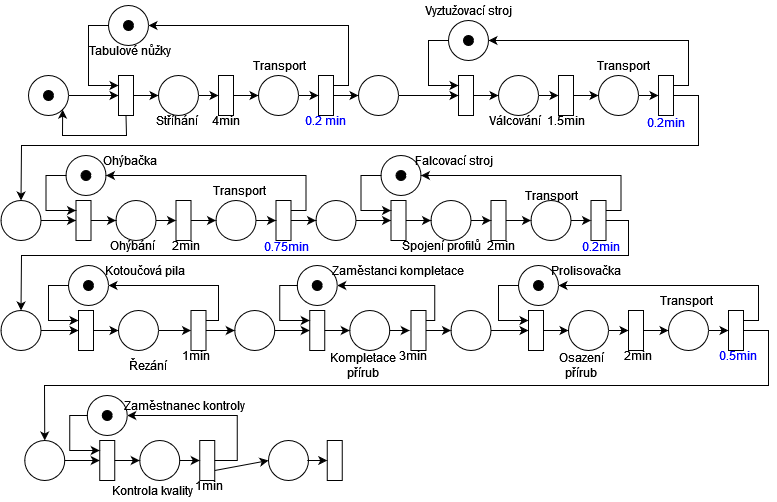
\includegraphics[width=17cm]{casy}
    \caption{Petriho síť s upraveným  rozmístěním pracovišť}
    \label{orig}
\end{figure}

\section{Architektura simulačního modelu/simulátoru}
Před počátkem simulace se inicializují kapacity jednotlivých zařízení. Při spuštění simulačního modelu je spuštěn vybraný experiment na základě parametrů příkazové řádky (bez zadaného parametru se spustí simulace výchozího modelu).

Vždy je simulováno 10 týdnů (pracovních hodin, ne čistého času, tedy 8 hodin * 7 dní * 10 týdnů) provozu a jedna jednotka modelového času značí jednu minutu reálného času. Na konci experimentu jsou vypsány informace o všech skladech\cite[str. 184]{ims} pracovních míst, a také histogram\cite[str. 81]{ims} celkového času zpracování výrobku.

Při zahájení experimentu je vytvořen a aktivován proces\cite[str. 171]{ims} reprezentující operaci stříhání\cite[str. 46]{bp} a případně procesy zaměstanců - přenašečů.
\newpage
\subsection{Namapování modelu}
Pro všechna pracoviště byla vytvořena třída pro generický proces \verb|Operation|, u nějž je možné měnit parametry tak, aby doba výroby a doba transportu vždy odpovídala jednotlivým operacím. Třída poskytuje jejím potomkům možnost implementovat metody pro inicializaci, počátek a konec operace. Z této třídy dědí veškeré další třídy reprezentující již jednotlivé operace (pracoviště).

Algoritmus průběhu generické operace:
\begin{algorithm}[ht]
		\SetKw{Break}{break}
        Zavolání vlastního inicializátoru(\texttt{MyConstructor})\;
        Čekání a poté zabrání volného pracoviště\;
        Zavolání metody počátku potomka(\texttt{MyStart})\;
        Čekání na dokončení práce\;
        Přičtení položek na odkladové místo pracoviště\;
		
		\eIf{Počet položek na odkladovém místě >= minimální počet nutný k transportu}
		{
			Čekání na dokončení transportu\;
			\For{pro počet položek na odkladišti}
			{
			    Zavolání ukončení operace (MyEnd)\;
			}
			Nastavení počtu položek na odkladišti na 0\;
		}{}
		Opuštění pracoviště\;
	

		\caption{Generický proces operace}
		\label{algorithm:workshift}
	\end{algorithm}
\begin{table}[H]
    \centering
    \begin{tabular}{|l|l|}
     \hline \textbf{operace} &  \textbf{třída}\\ \hline
Stříhání plechu   & CuttingOp\\ \hline
Z-profil    &  ZProfileOp\\ \hline
Ohýbání plechu    & BendingOp\\ \hline
Uzavírání profilu    & EnclosingOp\\  \hline
Řezání přírubových profilů    & Cutting2Op\\ \hline
Kompletace spojovacích přírub& CompletionOp\\ \hline
Osazení přírubami    & PlantingOp \\
    \hline
Kontrola kvality    &QualityAsOp \\
    \hline


    \end{tabular}
    \caption{Mapování operací na třídy}
    \label{rgrg}
\end{table}


\newpage
\section{Podstata simulačních experimentů a jejich průběh}
Obecným cílem experimentů bylo naýšení produkce, a tím i zisku, simulované firmy.

\subsection{Postup experimentování}
Nejdříve byly identifikovány potenciální cesty pro zvýšení produktivity. Každé takové cestě odpovídá jeden proběhlý experiment. Některé byly převzaty z neověřených tezí v literatuře, další se zaměřily na identifikaci problémů či zapojení nových metod do postupu výroby.

V průběhu experimentu byly použity metody půlení intervalu a záměrného naddimenzování některých hodnot.

\subsection{Jednotlivé experimenty}

\subsubsection{Validita výchozího modelu}
První experiment byl proveden nad modelem, simulujícím reálný stav výroby. Porovnáním jeho výstupů s realitou bylo provedeno ověření. Vzhledem ke shodnosti průměrného času výroby jednoho potrubí a výrobní kapacity lze model považovat za validní a pokračovat k dalším experimentům. V tomto experimentu nedochází k zahlcování a jednotlivá pracoviště jsou zatížena přibližně na 20 až 70 \%.



\subsubsection{Úzká místa}
Následným experimentem byla identifikována úzká místa ve výrobě - tedy stanoviště, která brzdí výrobu a na která musí následující stanoviště čekat. Hlavními ukazateli byly vytíženost stanoviště, tedy kolik procent času bylo využito, a velikost fronty, která se před ním tvořila.

Ve stavu odpovídajícím realitě je nejvíce vytíženo 1. pracoviště (stříhání plechu), díky čemuž další stíhají a nikde nevznikají fronty. Prvním logickým krokem tedy bylo navýšit produkitivitu tohoto stanoviště.

Jednoduchá simulace zdvojení tohoto stanoviště (tedy zakoupení 2. stejného stroje a přijmutí dalšího zaměstnance, či práce na jednom stroji na 2 směny) ukázala, že před stanicí pro kompletaci (3.) a osazování (4.) by se začaly tvořit fronty (které s postupem času jen narůstají).

Metodou půlení intervalu bylo následně zjištěno, že při zachování plynulosti celé výroby lze efektivitu stříhání plechu navýšit až o 41 \% (při vyšších hodnotách se již začnou tvořit stále se zvětšující fronty). Tím se celková produkce navýší o odpovídajících 41 \%.

\subsubsection{Nevyužitá práce}
Další experiment se zaobírá opačným problémem - identifikací pracovišť, která jsou málo využita a experimentováním, jak tento negavitní jev eliminovat.

Ve výchozím modelu jsou pracoviště \uv{řezání přírubových profilů} a \uv{kontrola kvality} nejméně využita - na 24, resp. 29 \%. Při snížení jejich výrobní kapacity na polovinu jsou stále využity jen na 47 a 59 \%. Z toho vyplývá, že zaměstnanci na těchto stanovištích mohou pracovat na poloviční úvazek - za udržení produktivity výroby a navýšení průměrného času výroby jedné trubky na TODO minut.


\subsubsection{Navrhovaná úprava rozmístění}
V tomto experimentu bylo simulováno nové rozmístění jednotlivých stanic podle návrhu v \cite[str. 51]{bp}. To bylo provedeno přenastavením časů pro transport mezi stanicemi dle zdroje. Následná simulace tohoto experimentu potvrdila zrychlení výroby jednoho kusu z 20 minut na 18.85 minut, což odpovídá zdroji.


\subsubsection{Dávkové předávání}
Cílem tohoto experimentu bylo zvýšit produkci tím, že polotovary budou přenášeny mezi stanicemi až po nahromadění určitého počtu kusů (v součastnosti se přenáší po jednom). Experiment byl spuštěn několikrát s různými počty kusů, po kterých jsou přenášeny. Každé pracoviště má vlastní překladiště, předání se tedy provede po jeho zaplnění, nezávisle na ostatních částech linky.

Předpoklad, že průměrná doba pro vyrobení jednoho kusu se zvětší, se potvrdil.


\subsubsection{Vyhrazený zaměstnanec pro přenos mezi pracovišti}
Tento experiment simuluje přijetí nového zaměstnance, jehož pracovní náplní by bylo pouze přenášet polotovary mezi jednotlivými stanovišti.

Nový zaměstnanec se řídí pro zjednodušení následujícím algoritmem: Zjistí, u kterého stanoviště je nahromaděno nejvíce polotovarů, a ty přenese.

Simulace chodu výroby s jedním takovým zaměstnancem ukázala, že produkce firmy by se zvýšila asi o 6 \%. Nový zaměstananec by tvořil 1/13, tedy cca 8 \%, zaměstanců, ovšem potřeboval by prakticky nulovou kvalifikaci a tedy nižší mzdu, jeho zařazení by tudíž mohlo být pro firmu výhodné.

Vedlejším efektem zařazení pomocného pracovníka bylo zvýšení průměrné doby výroby jednoho produktu, a to o více než dvojnásobek. Tato veličina ovšem ovlivňuje pouze dobu náběhu ze zastavení do plné produkce.

%mnohem méně důležitá, než počet vyprodukovaných výrobků za dobu simulace.

V experimentu s více zaměstnanci pro přenášení se již produkce téměř nezvýšila, pouze se zanedbatelně snížil průměrný čas výroby jednoho produktu, stále však nedosáhl na hodnotu bez přenašečů.

\subsection{Závěry experimentů}
Bylo provedeno TODO experimentů, z nichž lze odvodit efektivitu a výhodnost použití navrhovaných vylepšení v reálné výrobě.

\section{Shrnutí simulačních experimentů a závěr}
Z provedených experimentů vyplývá, že

\newpage
\bibliographystyle{czechiso}
\bibliography{ims}

\end{document}
